\chapter{Metodologie}
\label{teoria}
Nel corso di questo capitolo saranno introdotti progressivamente i concetti principali su cui si fonda la \textit{computer vision} (visione artificiale) e il \textit{machine learning} (apprendimento automatico). Questi contenuti permetteranno di comprendere da un punto di vista teorico quanto descritto nella sezione sperimentale della tesi (cap. \ref{esperimenti}).

Per i primi paragrafi, dedicati all'\textit{image processing}, le principali fonti seguite sono \cite{gianvito} e \cite{computerVision}.

Per i paragrafi dedicati al \textit{machine} e \textit{deep learning} le fonti di riferimento sono \cite{dlbook} e soprattutto \cite{cs231n}.


\section{Immagini digitali}
\label{imDig}
Caratterizziamo intuitivamente il concetto di "immagine" dal punto di vista informatico.

Un'\textbf{immagine digitale} è una rappresentazione binaria di un'immagine (in generale a colori) a due dimensioni\footnote{Ci riferiamo in questa sede solo alle immagini di tipo raster, quelle cioè con risoluzione e numero di canali di colore fissati a priori, come ad esempio le immagini digitali in formato jpg.}; essa può essere definita matematicamente come un tensore $\mathcal{I}\in\{0,\dots,255\}^{h\times w\times c}$, dove $h$ e $w$ sono rispettivamente dette \textbf{altezza} e \textbf{larghezza} dell'immagine, la coppia $(w,h)$ \textbf{risoluzione} mentre $c$ è il numero di \emph{canali di colore}\footnote{Spesso si scrive che $\mathcal{I}$ è un immagine $w\times h\times c$, o più semplicemente $w\times h$ (assumendo $c=3$)}. Nello \textbf{spazio di colore sRGB} (standard RGB, d'ora in avanti abbreviato in RGB), ampiamente adoperato, i canali di colore sono rosso (R, Red), verde (G, Green) e blu (B, Blue), quindi $c=3$. In mancanza di diverse indicazioni, ci si riferirà nel seguito allo spazio di colore RGB.

Un \textbf{pixel} $p(i,j)$ è definito come la funzione vettoriale
\[p(i,j)=[r(i,j),g(i,j),b(i,j)]\]
essendo $r,g,b:\{0,\dots,h\}\times\{0,\dots,w\}\to\{0,\dots,255\}$ le funzioni scalari che associano ad ogni posizione bidimensionale $i,j$ dell'immagine un valore intero di \textbf{intensità luminosa} compreso tra 0 e 255, uno per ciascuno dei tre canali RGB.
Ogni pixel definisce univocamente un colore nello spazio RGB, il quale può quindi rappresentare in tutto $256^{3}$ colori diversi, cioè circa 17 milioni.

Si può immaginare il tensore immagine $\mathcal{I}$ come una "pila" di tre matrici, una per ogni canale di colore, come mostrato in figura \ref{fig:rappresentazione_tensore}.

\begin{figure}[h]
\centering
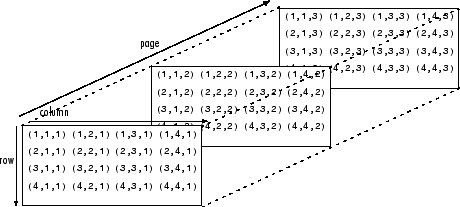
\includegraphics[scale=0.7]{rappresentazione_tensore}
\caption{Rappresentazione grafica di un tensore tridimensionale; in ogni posizione compaiono gli indici del tensore}
\label{fig:rappresentazione_tensore}
\end{figure}

Un esempio di immagine digitale, scomposta nelle sue componenti RGB, è mostrato in figura \ref{fig:canali_rgb}.

\begin{figure}[h]
  \begin{minipage}[b]{0.46\textwidth}
    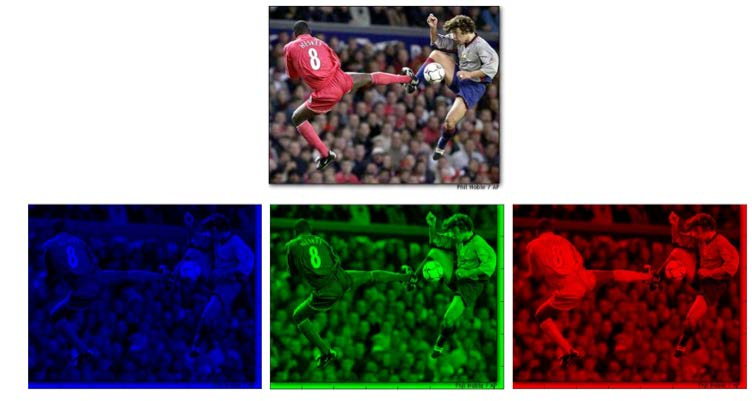
\includegraphics[width=\textwidth]{canali_rgb}
    \caption{Canali RGB di un'immagine}
    \label{fig:canali_rgb}
  \end{minipage}
  \hfill
  \begin{minipage}[b]{0.46\textwidth}
    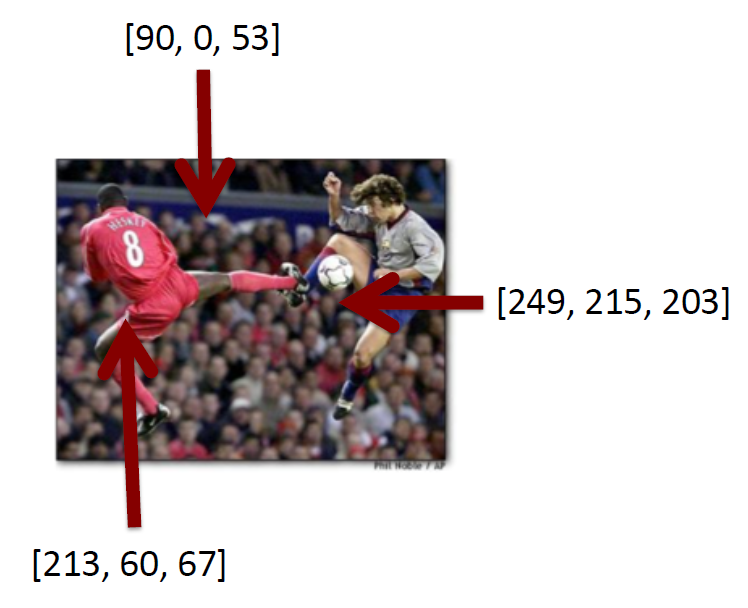
\includegraphics[width=\textwidth]{pixel}
    \caption{Pixel di un'immagine}
  \end{minipage}
\end{figure}

In Matlab un'immagine digitale può essere rappresentata con il tipo di dato \verb|multidimensional-array| con tre dimensioni (corrispondenti ai tre canali di colore RGB), in cui ciascun elemento è di tipo \verb|uint8| (ma può appartenere anche ad altri tipi di dato\footnote{\url{https://it.mathworks.com/help/matlab/ref/image.html?s_tid=doc_ta#buqdlnb-C}}).

È possibile importare un'immagine RGB con la funzione:
\begin{verbatim}
im = imread("immagine.jpg");
\end{verbatim}
I canali Rosso \verb|R|, Verde \verb|G| e blu \verb|B| possono essere ottenuti come:
\begin{verbatim}
R = im(:,:,1);
G = im(:,:,2);
B = im(:,:,3);
\end{verbatim}
Il pixel di posizione $(i,j)$ è quindi:
\begin{verbatim}
p = [im(i,j,1) im(i,j,2) im(i,j,3)];
\end{verbatim}

\subsection{Spazio di colore Lab}
Oltre al modello RGB descritto al paragrafo precedente, esistono ulteriori spazi di colore che consentono di ottenere una differente rappresentazione delle medesime tonalità dei pixel.
Nel presente lavoro di tesi (par. \ref{faseRitaglio}) si utilizza una conversione delle immagini dallo spazio di colore iniziale RGB allo spazio di colore \textbf{CIE 1976 L*a*b*} (nel seguito abbreviato come Lab).
Nello spazio Lab le tonalità sono ancora espresse da triplette di valori (L*, a* e b*), ma con un significato diverso rispetto a RGB: il valore L* rappresenta la luminanza
(variazione di luminosità), mentre le altre due rappresentano la crominanza (variazione
di colore), rispettivamente una scala verde-rosso (a*) ed una scala blu-giallo (b*).

A partire dall’immagine \verb|im| è possibile convertire lo spazio di colori da RGB a Lab, ottenendo una nuova immagine \verb|im_lab|:
\begin{verbatim}
im_lab = rgb2lab(im);
\end{verbatim}
I dettagli sulla conversione di spazio di colore possono essere letti al par. 2.1.1 di \cite{gianvito}.

\subsection{Collezioni di immagini in Matlab}
\label{datastore}
Una delle necessità principali del lavoro affrontato è stata la gestione di grandi quantità di immagini. Si riportano i tipi di dato messi a disposizione da Matlab e utilizzati negli esperimenti del presente lavoro di tesi:

\begin{itemize}

\item \verb|imageDatastore|: oggetto progettato appositamente per gestire ed elaborare rapidamente una grande quantità di immagini. Per istanziare un oggetto \verb|imageDatastore| bisogna specificare l'argomento \verb|path| che indica il percorso della collezione di immagini da importare. Altri argomenti (coppie argomento-valore) opzionali per l'inizializzazione di questo oggetto sono:
\begin{itemize}
\item \verb|’IncludeSubfolders’,true|\\
Include le immagini contenute nelle sottocartelle di \verb|path| 
\item \verb|’LabelSource’,’foldernames’|\\
Assegna a ciascuna immagine un’etichetta
data dal nome della cartella in cui è contenuta
\end{itemize}
Quindi, per creare l'oggetto:
\begin{verbatim}
imds = imageDatastore(path,’IncludeSubfolders’,true,...
’LabelSource’,’foldernames’);
\end{verbatim}
L’elenco delle immagini è restituito nel campo \verb|imds.Files|.

\item \verb|augmentedImageDatastore|: oggetto creato a partire da un \verb|imageDatastore| applicando operazioni di preprocessing e augmentation specificate in un oggetto \verb|imageDataAugmenter|. La sintassi di questo oggetto verrà approfondita nel par. \ref{augmentation}.

\end{itemize}

\section{Trasformazioni}
\label{trasformazioni}
Si riportano le operazioni fondamentali che hanno consentito, nel presente lavoro di tesi, di trasformare le immagini in una forma maggiormente adatta ad un’analisi successiva, una strategia chiamata \textit{image augmentation} (par. \ref{augmentation}).

\subsection{Ridimensionamento}
Il ridimensionamento consente, in generale, di ottenere una nuova immagine a risoluzione differente, riducendo o aumentando il numero di pixel utilizzati per rappresentarla.
Nel caso del presente lavoro, le dimensioni delle immagini sono state ridotte (par. \ref{faseRitaglio}), per diminuire il costo computazionale delle operazioni successive.
Per ridimensionare un'immagine \verb|im| in Matlab si può usare la funzione \verb|imresize|\footnote{La funzione imresize attua, per lo scopo, una tecnica avanzata di calcolo numerico: l’interpolazione bicubica. (par. 2.2.1 di \cite{gianvito} per i dettagli.)}, specificando la nuova lunghezza \verb|w'| e la nuova altezza \verb|h'|:
\begin{verbatim}
im_res = imresize(im,[h' w']);
\end{verbatim}

\subsection{Rotazione}
La rotazione di un'immagine digitale può essere effettuata calcolando per ogni suo pixel $(x,y)$ il prodotto matriciale
\begin{equation*}
\begin{bmatrix}
x' \\
y'
\end{bmatrix} = 
\begin{bmatrix}
\cos\alpha & -\sin\alpha \\
\sin\alpha & \cos\alpha
\end{bmatrix}
\begin{bmatrix}
x \\
y
\end{bmatrix}
\end{equation*}
in cui $\alpha$ è l’angolo di rotazione misurato in senso antiorario rispetto all’asse x e $(x',y')$ le coordinate del pixel trasformato. L'immagine ruotata è l'insieme dei pixel $(x',y')$ calcolati.

In Matlab, la rotazione di un'immagine \verb|im| di un angolo \verb|a| può essere effettuata con
\begin{verbatim}
rotated = imrotate(im, a);
\end{verbatim}

\subsection{Riflessione}
La riflessione rispetto all’asse x di un'immagine digitale può essere effettuata calcolando per ogni suo pixel $(x,y)$ il prodotto matriciale
\begin{equation*}
\begin{bmatrix}
x' \\
y'
\end{bmatrix} = 
\begin{bmatrix}
1 & 0 \\
0 & -1
\end{bmatrix}
\begin{bmatrix}
x \\
y
\end{bmatrix}
\end{equation*}
dove $(x',y')$ sono le coordinate del pixel trasformato. L'immagine riflessa è l'insieme dei pixel $(x',y')$ calcolati.

In Matlab, la riflessione di un'immagine \verb|im| rispetto all'asse x può essere effettuata con
\begin{verbatim}
flipped = flipdim(im, 2);
\end{verbatim}

\subsection{Traslazione}
La traslazione orizzontale, a differenza delle precedenti operazioni, è una trasformazione affine ma non lineare, quindi
la rappresentazione con le matrici richiede il passaggio ad un diverso tipo di coordinate
dette omogenee:
\begin{equation*}
\begin{bmatrix}
x&y
\end{bmatrix}^\top \mapsto
\begin{bmatrix}
x&y&1
\end{bmatrix}^\top
\end{equation*}
A questo punto, è possibile ottenere le nuove coordinate traslate $(x', y')$ calcolando:

\begin{equation*}
\begin{bmatrix}
x'\\y'\\1
\end{bmatrix} = 
\begin{bmatrix}
1 & 0 & t_x \\0 & 1 & t_y \\0 & 0 & 1
\end{bmatrix}
\begin{bmatrix}
x \\ y \\ 1
\end{bmatrix}
\end{equation*}

In Matlab, la traslazione orizzontale di \verb|t| pixel di un'immagine \verb|im| può essere effettuata con
\begin{verbatim}
translated = imtranslate(im,[t 0]);
\end{verbatim}
dove \verb|t|>0 implica una traslazione verso destra, \verb|t|<0 verso sinistra.\\

I risultati delle quattro trasformazioni finora viste sono visualizzate in figura \ref{fig:trasformazioni}

\begin{figure}[h]
\centering

\begin{subfigure}[b]{\textwidth}
\centering
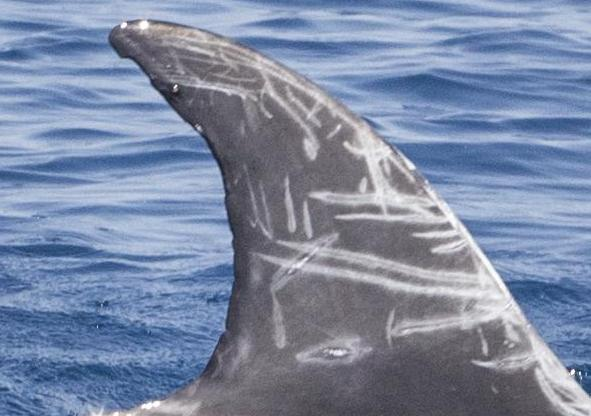
\includegraphics[width=0.24\textwidth]{pinnaOriginale}
\caption{Immagine originale}
\end{subfigure}

\begin{subfigure}[b]{0.24\textwidth}
\centering
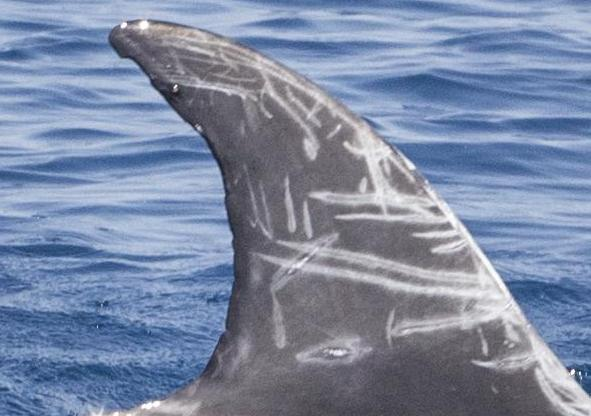
\includegraphics[width=0.4\textwidth]{pinnaOriginale}
\caption{Ridimensionata}
\end{subfigure}
\begin{subfigure}[b]{0.24\textwidth}
\centering
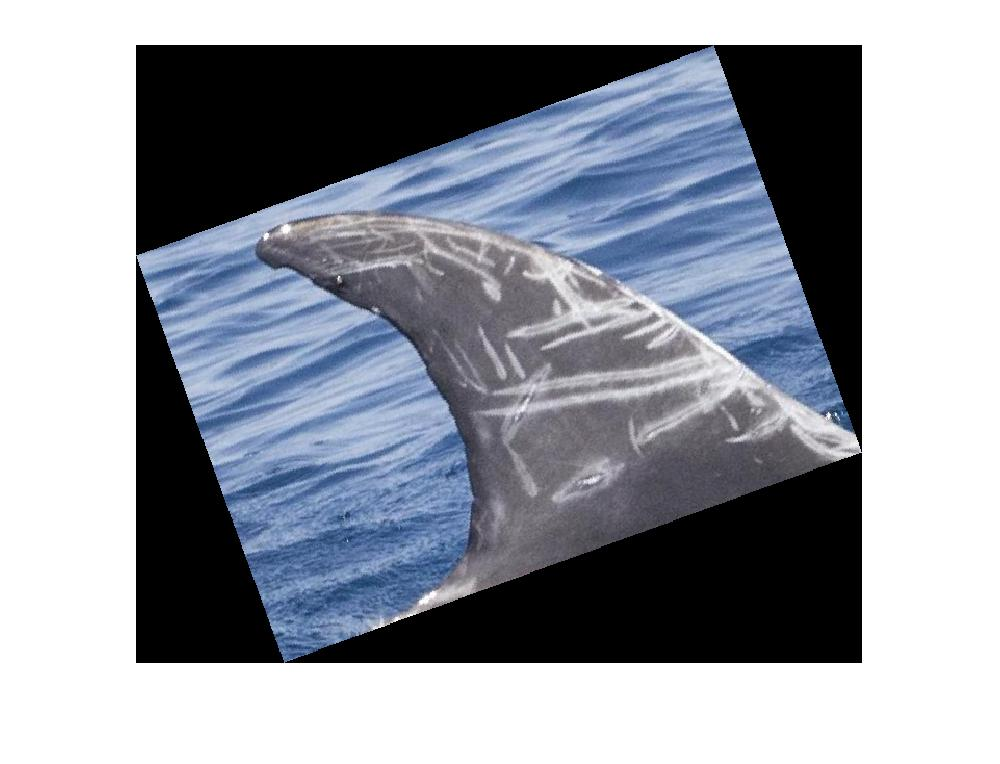
\includegraphics[width=\textwidth]{pinnaRuotata}
\caption{Ruotata di 20$^\circ$}
\end{subfigure}
\begin{subfigure}[b]{0.24\textwidth}
\centering
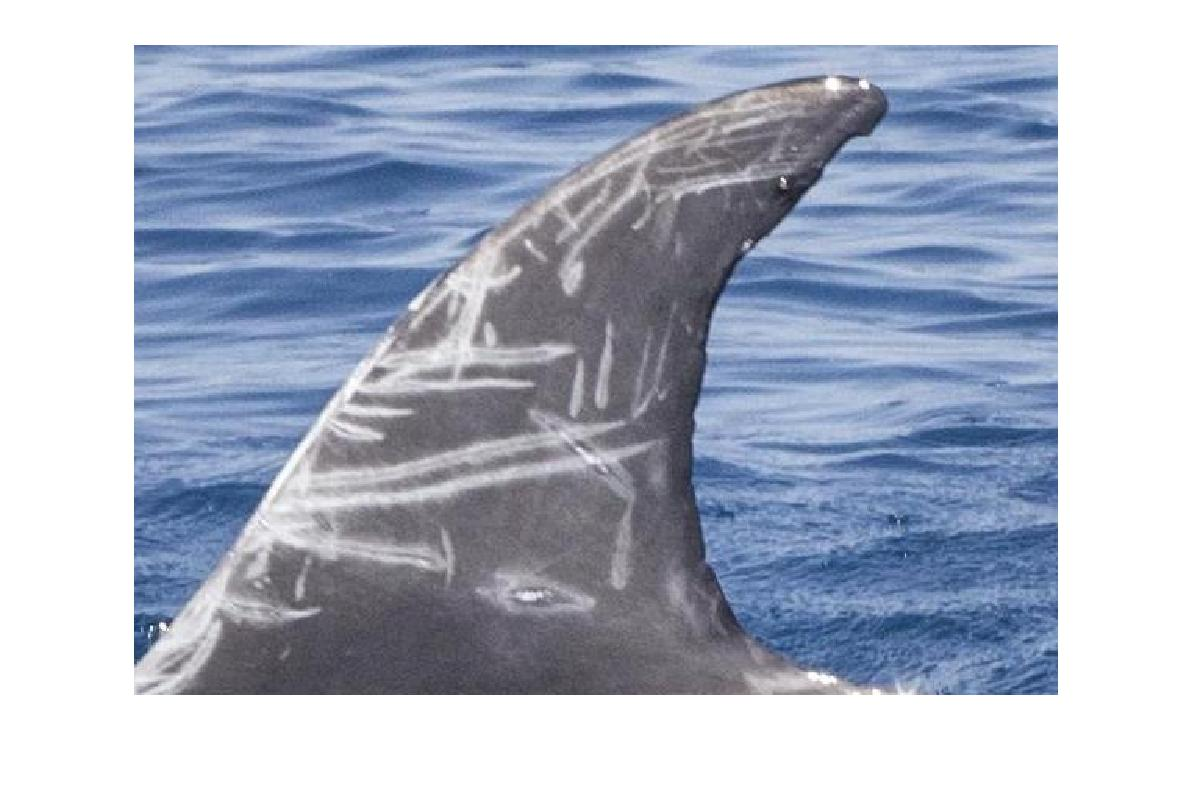
\includegraphics[width=\textwidth]{pinnaRiflessa}
\caption{Riflessa}
\end{subfigure}
\begin{subfigure}[b]{0.24\textwidth}
\centering
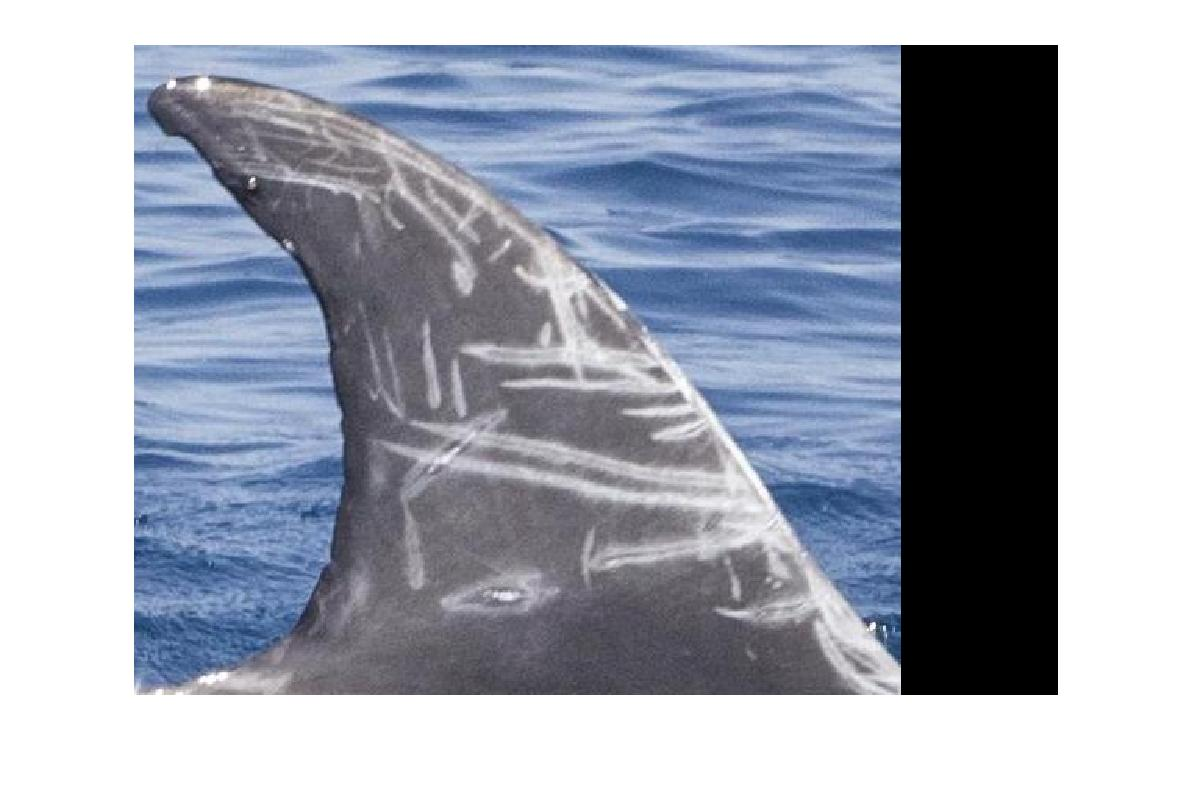
\includegraphics[width=\textwidth]{pinnaTraslata}
\caption{Traslata di -100px}
\end{subfigure}

\caption{Trasformazioni applicate ad un'immagine digitale}
\label{fig:trasformazioni}
\end{figure}

\subsection{Convoluzione}
\label{convoluzione}
Nell’ambito dell’\textit{image processing} esiste una quantità notevole di operatori definiti "locali", che operano cioè non su un singolo pixel ma su un gruppo di pixel contigui.
L’operatore locale maggiormente usato è l’operatore di convoluzione. Nell'ambito del presente lavoro, esso ha un'importanza centrale per la \textit{feature extraction} delle immagini, all'interno delle reti neurali convoluzionali (par. \ref{CNN}), e più specificamente nei layer convoluzionali (par. \ref{CONV}).


Nel seguito si presenta, pertanto, una definizione rigorosa dell'operazione di convoluzione e si forniscono semplici esempi di implementazione.

Dati due segnali discreti $x(k)$ e $w(k)$, si definisce \textbf{(somma di) convoluzione tra $x$ e $w$} una nuova funzione $s(k)$ definita come \begin{equation*}
s(k)=x(k)\ast w(k)\eqdef \sum_{i=-\infty}^{+\infty}x(i)w(k-i), i\in\Z
\end{equation*}

Si dimostra che questa operazione gode della proprietà commutativa, associativa e distributiva rispetto alla somma.

Nell'ambito della \textit{computer vision} si utilizza una versione multidimensionale dell'operazione di convoluzione, utilizzando la seguente terminologia:
\begin{itemize}
\item il primo segnale $x$ è detto \textbf{input}, generalmente costituito da un'immagine od una sua elaborazione;
\item il secondo segnale $w$ è detto \textbf{filtro} o \textbf{kernel}, solitamente costituito da una matrice
di dimensioni ridotte rispetto all'input;
\item il risultato $s$ è detto \textbf{feature map}, poiché l'operazione di convoluzione è spesso utilizzata per l'estrazione di feature a partire dall'input (par. \ref{CONV}).
\end{itemize}
È ovvio che la somma di infiniti termini prevista dalla definizione di convoluzione con segnali discreti si riduce ad una somma limitata alle dimensioni dell'immagine. Nel caso in cui l'input sia una matrice bidimensionale, ad esempio un'immagine in scala di grigi $I\in\R^{h\times w}$, anche il kernel impiegato è solitamente una matrice bidimensionale di dimensioni ridotte $K\in\R^{a\times b}$, ottenendo l’operazione:
\begin{equation*}
s(i,j)=(I\ast K)(i,j)=\sum_{k=1}^a\sum_{r=1}^b I(i+k-1,j+r-1)K(l-k+1,w-r+1)
\end{equation*}

Molte librerie, in realtà, implementano la convoluzione attraverso la funzione di crosscorrelazione (indicata con $\oast$).
In tal caso ciascun elemento della feature map si ottiene come
\begin{equation*}
s(i,j)=(I\oast K)(i,j)=\sum_{k=1}^a\sum_{r=1}^b\mathcal{I}(i+k-1,j+r-1)K(k,r)
\end{equation*}
L'operazione appena esposta - che si dimostra essere equivalente ad una convoluzione tra $I$ e $K$ - ha una semplice interpretazione, visualizzata in fig. \ref{fig:interpretazioneConvoluzione}. Convolvere un'immagine con un kernel equivale a far scorrere la matrice che rappresenta il kernel lungo l'immagine, e sviluppare i prodotti \textit{element-wise} (termine a termine) e sommarli tra loro, ottenendo l'elemento della feature map.

\begin{figure}[h]
\centering
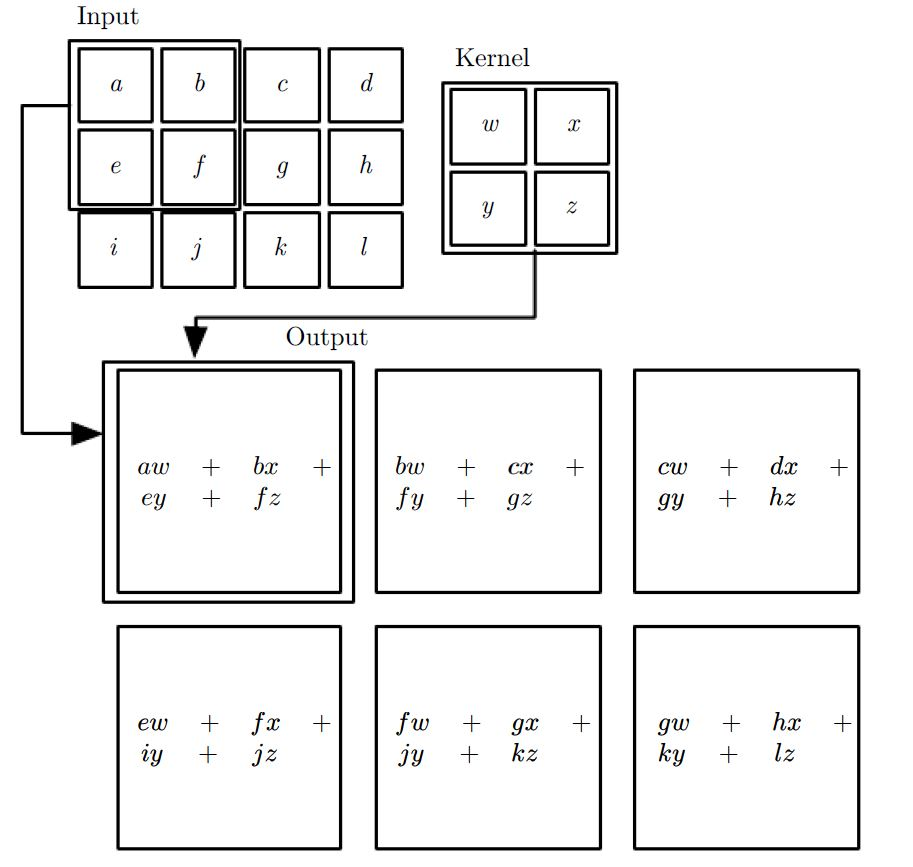
\includegraphics[width=0.5\textwidth]{interpretazioneConvoluzione}
\caption{Un esempio di cross-correlazione (ovvero convoluzione discreta 2-D senza il
ribaltamento del kernel)}
\label{fig:interpretazioneConvoluzione}
\end{figure}

Nel caso (più comune) in cui l’input sia un tensore (ad esempio un’immagine a colori) $\mathcal{I}\in\R^{h\times w\times c}$ si richiede che il kernel abbia lo stesso numero $c$ di livelli, ad esempio $\mathcal{K}\in\R^{a\times b\times c}$. L'operazione viene così ridefinita.
\begin{equation*}
s(i,j)=(\mathcal{I}\oast\mathcal{K})(i,j,k)=\sum_{k=1}^a\sum_{r=1}^b\sum_{s=1}^c\mathcal{I}(i+s-1,j+r-1,k)K(r,s,k)
\end{equation*}
Come si nota, la feature map ottenuta sarà sempre bidimensionale (a prescindere dalla profondità $c$ del tensore in input).

Completeremo la trattazione sulla convoluzione nel par. \ref{CONV} sul layer convoluzionale di una CNN.

\section{Problemi di \textit{Computer Vision}}
\label{computerVision}
In questa sezione si riportano alcuni problemi caratteristici della \textit{computer vision}, affrontati nel corso del lavoro e finalizzati ad una comprensione di alto livello del contenuto delle immagini (e dei video) da parte del computer. Il nome italiano della disciplina, "visione artificiale", richiama in questo senso l'obiettivo di rendere artificiali i compiti svolti dal sistema visivo umano.

\subsection{Object recognition}
\label{objectRecognition}
L'\textbf{\textit{object recognition}} (in italiano: riconoscimento di oggetti) nell'ambito della visione artificiale è il problema di assegnare una descrizione testuale o una o più etichette ad un'immagine, tipicamente sulla base di uno o più determinati oggetti che un computer riesce a riconoscere all'interno di essa.

Ogni categoria esistente di oggetti ha delle caratteristiche fondamentali che la differenziano da qualunque altra categoria di oggetti. Attraverso tecniche di \textit{machine learning} è possibile ricavare una descrizione di una certa categoria addestrando la macchina a riconoscere le caratteristiche (\textit{features}) fondamentali di quella categoria di oggetti, a partire da un insieme di immagini campione afferenti a quella categoria.

Per rendere affidabile il riconoscimento, è importante che l'insieme di caratteristiche estratte da ogni immagine campione sia insensibile a variazioni del punto di vista, di scala, delle condizioni di illuminazione, alle distorsioni geometriche, all'occlusione dell'oggetto, al \textit{clutter} (ingombro) di altri oggetti non informativi sullo sfondo, alle variazioni intra-classe dell'oggetto, come mostrato in fig. \ref{fig:variabilita}.

\begin{figure}[h]
\centering
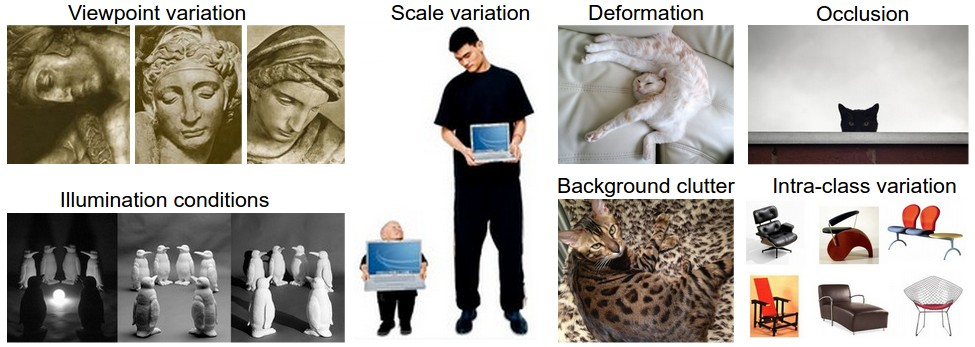
\includegraphics[width=0.9\textwidth]{variabilita}
\caption{I principali "ostacoli" al riconoscimento automatico degli oggetti} 
\label{fig:variabilita}
\end{figure}

L'uomo riconosce una moltitudine di oggetti in immagini con poco sforzo, nonostante i fattori di variabilità descritti. Questo compito è ancora una sfida aperta per la computer vision in generale.\\

Il problema dell'\textbf{\textit{image classification}} è uno specifico problema di \textit{object recognition} che consiste nell'assegnare una singola etichetta (o una distribuzione di probabilità su più etichette) ad un'immagine da un insieme fisso di etichette (anche dette "categorie" o "classi"). In fig. \ref{fig:imageClassification} è visualizzato il problema in esame.

\begin{figure}[h]
\centering
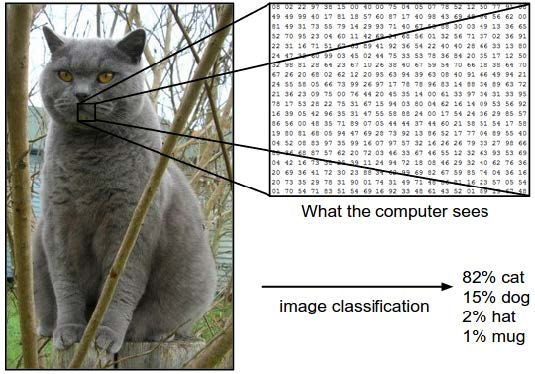
\includegraphics[width=0.7\textwidth]{imageClassification}
\caption{Il task della \textit{image classification} consiste in questo caso nel calcolare una distribuzione di probabilità su quattro etichette (gatto, cane, cappello, tazza) per un'immagine digitale.} 
\label{fig:imageClassification}
\end{figure}

In letteratura sono stati proposti numerosi metodi per la risoluzione efficiente dei task di \textit{object recognition}, attraverso l'impiego di diverse tecniche di \textit{machine learning} (ad esempio l'algoritmo di clustering \textit{k-Nearest Neighbor}). Negli ultimi anni i risultati più promettenti sono stati offerti dalle \textit{reti neurali convoluzionali}, di cui parleremo diffusamente nel seguito del capitolo (par. \ref{CNN}) e che verranno impiegate negli esperimenti (par. \ref{faseClassificazione}).

\subsection{Object detection}
\label{objectDetection}
Un altro importante problema di \textit{computer vision} è l'\textbf{\textit{object detection}} (in italiano: rilevamento di oggetti). Esso consiste nella localizzazione di oggetti di categorie stabilite a priori ed in seguito (o talvolta in contemporanea) la loro classificazione, per mezzo di un opportuno modello di classificazione.

Il compito si rivela, evidentemente, più difficile di quello della semplice classificazione di oggetti, essendo la localizzazione degli oggetti all'interno dell'immagine un problema anch'esso non banale.\\

L'obiettivo di questo lavoro di tesi è la risoluzione di una particolare istanza (\textit{task}) di \textit{object detection}: si vogliono identificare, localizzare e conseguentemente ritagliare, le eventuali porzioni di un'immagine contenenti pinne dorsali di delfini. La classe di oggetti di interesse è quindi una sola.

Grazie al dominio ristretto del problema in esame, il task di rilevamento è risolto con un approccio in due fasi:
\begin{itemize}
\item dapprima, si localizzano e si ritagliano le eventuali pinne presenti nell'immagine, sfruttando una forma di conoscenza di alto livello direttamente disponibile nella rappresentazione delle immagini: il colore\footnote{L'idea di sfruttare il colore per isolare le pinne dei cetacei deriva proprio dalla differenza di tonalità tra l'acqua (tendente al blu e al verde) e le pinne (tendenti al grigio)};
\item in seguito, i ritagli sono sottoposti ad una fase di classificazione, che ne conferma la natura di 'Pinna' o ne smentisce il contenuto informativo ('No pinna').
\end{itemize}
Si rimanda direttamente al cap. \ref{esperimenti} per la descrizione degli esperimenti condotti.

\subsection{ImageNet Database e ILSVRC}
\label{imagenet}
\textbf{\textit{ImageNet}} è un'ampia base di dati di immagini, realizzata per l'utilizzo nel campo dell'\textit{object recognition} \cite{imagenet}. Il dataset consiste in più di 14 milioni di immagini con diverse risoluzioni che sono state annotate manualmente con l'indicazione degli oggetti in esse rappresentati e, per circa un milione di esse, della bounding box che li delimita. Gli oggetti individuati sono stati classificati in più di 22.000 categorie. Alcune categorie di oggetti frequenti, come ad esempio "pallone" o "fragola", consistono di diverse centinaia di immagini.
Le immagini sono state raccolte nel web ed etichettate manualmente tramite il tool di crowd-souring Amazon’s Mechanical Turk.\\

A partire dal 2010, ogni anno viene indetta una competizione di \textit{object recognition} e \textit{detection} denominata \textbf{\textit{ImageNet Large Scale Visual Recognition Challenge}} (ILSVRC): in tale occasione programmi software vengono fatti competere per classificare e rilevare correttamente oggetti e scene contenuti nelle immagini.

Nell'ambito della competizione viene impiegata un sottoinsieme di immagini del database ImageNet, con immagini appartenenti a 1000 categorie e circa 1000 immagini per ciascuna categoria. In tutto ci sono circa 1.2 milioni di immagini per l'addestramento dei modelli, 50.000 per la validazione e 150.000 per il testing.

Per i classificatori che competono nella ILSVRC le prestazioni vengono misurate sulla base di due parametri:
\begin{itemize}
\item \textit{top-5 error}: la frazione di immagini del test set per le quali la classe corretta non è tra le cinque classi considerati le più probabili dal modello
\item \textit{top-1 error}: la frazione di immagini del test set classificate in maniera errata dal modello
\end{itemize}

Le tre reti neurali convoluzionali scelte per effettuare gli esperimenti presentati in questo lavoro sono risultate vincitrici della ILSVRC 2012 (Alexnet, par. \ref{alexnet}), ILSVRC 2014 (GoogLeNet, par. \ref{googlenet}) e ILSVRC 2015 (ResNet, par. \ref{resnet}).
